
\section{Behavioural data}\label{sec:behavioural_data}
%[1/f POWER SPECTRUM]
\subsection{Neural frequency bands}\label{subsec:neur_freq_bands}
Throughout much of this thesis, links are drawn between timescales of interactions and dynamics in the FNS model and well-studied frequency bands of activity in the human brain. It is then valuable to outline the studied computational and functional interpretations of such frequency bands. Neural firing activity is divided into frequency bands named by greek letters, originally discovered and decomposed from electroencephalogram (EEG) data. Divisions are only approximate, but for this thesis these bands are: delta (0.1 - 4~Hz), theta (4 - 8~Hz), alpha (8 - 14~Hz), beta (14 - 30~Hz), and gamma (30 - 220~Hz) \cite{fan_relation_2007, klimesch_frequency_2018}. Of particular interest to this thesis are the interpretations of theta and gamma neural activity as functionally important to attention and search tasks of computation. Theta rhythms have been shown to modulate attention during auditory tasks \cite{wang_attention_2022, yang_neural_2024}, visual search tasks \cite{kawashima_attentional_2022, spyropoulos_theta_2018, Mo_competing_2019}, and in analysing the general attentional mechanism of the brain \cite{tan_theta_2024, fan_relation_2007, klimesch_frequency_2018}. Intervals between theta peaks are finding stronger interpretation in the neuroscience literature as discretely sampling the environment for integration into the internal model of the brain. Strong direct evidence for this theory include correlations between intelligence and high theta peak power in EEG data during tasks requiring focus and attention \cite{wang_attention_2022, tan_theta_2024}, and the discovered sensitivity of the visual system to react and search scenes on a theta rhythm \cite{kawashima_attentional_2022, spyropoulos_theta_2018}. Accordingly, the firing patterns which define the lowest level of information carried in the brain are regularly found to be gamma in scale ($\sim 30-100$~Hz) \cite{canolty_high_2006, harris2026-cn, ursino_thetagamma_2024, brooks_thetagamma_2020, tort_thetagamma_2009}. 

\begin{figure}
    \centering
    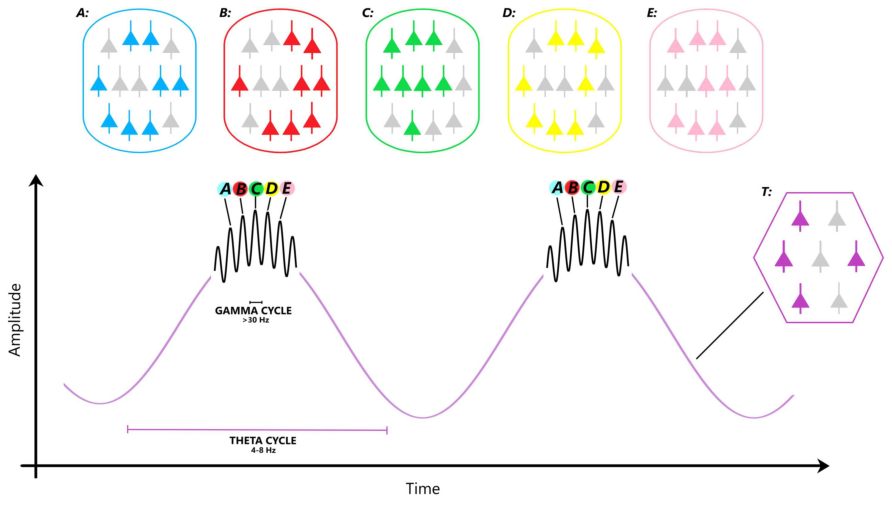
\includegraphics[width=0.6\linewidth]{figures/Theta_Gamma_Coupling_image.pdf}
    \caption{\textbf{A schematic representation of theta-gamma coupling (TGC).} TGC has it's foundations in the work of Lisman and Jensen in correctly ordering neural signals \cite{lisman_theta-gamma_2013}, and subsequently expanded and used to describe the dynamic mechanism the brain uses during exploration to modulate close attention upon individual centres of focus \cite{mclelland_theta-gamma_2016}. \textit{Schematic adapted from figure~2 of M. Ursino and G. Pirazzini, 2024 \cite{ursino_thetagamma_2024}}}
    \label{fig:placeholder}
\end{figure}
\subsection{Gaze trajectories}\label{subsec:gaze_traj}
Healthy human gaze trajectories consist of different dynamical regimes. The most studied property of the pattern of gaze trajectories are their division into periods of fixation, interspersed by near-instantaneous jumps between fixations, these jumps being known as ``saccades'' \cite{erkelens_coordination_2006, seung_how_1996, lencastre_dynamical_2025, benitezy_eyetracking_1970}. Importantly, this behaviour of local movements interspersed with large discontinuous jumps suggest modelling eye movements through a Lévy flight. This method has a limited history in the literature, and fitting data to a simple phenomenological Lévy flight parametrised by the stable parameter $\alpha$ found limited use as a biomarker for ADHD \cite{papanikolaou_levy_2024}. Saccade metrics in general have been found to be valuable as non-invasive biomarkers for broader neural disorders, including schizophrenia, autism, ADHD, OCD, bipolar disorder, Parkinson's disease, and multiple sclerosis \cite{morita_eye_2017, bittencourt_saccadic_2013,zhu_diagnosis_2024, caldani_saccadic_2017, wang_saccadic_2025}. Periods of fixation have received less scholarly attention as a biomarker of cognition. Gaze fixations exhibit three distinct dynamical patterns: near-instant microsaccades within the same point of focus, slow ocular drift about a point of focus, and high frequency ocular micro tremor \cite{van_ede_looking_2026,graham_ocular_2023, engbert_integrated_2011, spauschus_origin_1999}. Examinations and literature reviews of these behaviours have often not considered their computational role in active sensing and efficient search.
